% !TEX program = lualatex
% !TEX TS-program = lualatex
% !BIB program = bibtex
% !BIB TS-program = bibtex
% example.tex -- the worked example; write your own document in main.tex.
% Build: make -f Makefile.a11y example
% First block of every accessible document, above \documentclass. lang sets
% /Lang; pdfstandard=ua-2 gives PDF 2.0 + the PDF/UA-2 flag; check-tagging-status
% appends a package report to the .log that `make -f Makefile.a11y check` reads.
% pdfstandard=a-4f adds archiving: an embedded sRGB output intent and the Print
% flag on every link annotation, so the underline survives printing. It empties
% the document information dictionary, so the title travels in XMP alone.
% Meets: ISO 14289-2:2024 8.11 (metadata); ISO 19005-4:2020 (PDF/A-4f).
\DocumentMetadata{
  lang        = en-US,
  pdfstandard = ua-2,
  pdfstandard = a-4f,
  tagging     = on,
  check-tagging-status,
}
\documentclass{clemsona11y}


% The packages below are all compatible with tagging. --------------------------

\usepackage{booktabs}   % rules for the tables below; optional
% The packages for the examples below. None appears in section 1 (unsupported) or
% 2 (incompatible) of the tagging status report, and each produces Formula, list
% or Figure tags. Meets: LaTeX tagging status list, sections 1-2 (none listed).
\usepackage[version=4]{mhchem} % chemical formulae and reactions
\usepackage{siunitx}        % numbers and units (do not load physics as well)
\usepackage{braket}         % bra-ket notation
\usepackage{algpseudocode}  % the steps of an algorithm
\usepackage{tikz}           % a diagram drawn in the document
% A long \verb string or URL cannot be hyphenated and can end up in the margin;
% \emergencystretch lets TeX loosen such a line instead (typography, not tagging).
\setlength{\emergencystretch}{2em}

% ------------------------------------------------------------------------------

% pdftitle: doubled braces keep commas in one title. pdfauthor: commas between names.
\title[pdftitle={{Accessible LaTeX, quickly}}]{Accessible LaTeX, quickly}
\author[pdfauthor={First Author, Second Author}]{First Author and Second Author}
\date{\today} % Can be left blank; the class adds \today to the PDF metadata.
\begin{document}
\maketitle

\begin{abstract}
This file is a working example of every kind of content a paper or a report usually holds:
headings, text, notes, cross-references, mathematics, chemistry, units, algorithms, figures
with alt text and long descriptions, tables and an appendix. All of it is tagged, so the PDF
conforms to PDF/UA-2. Copy the pieces you need; the comments in the source say why each line
is written the way it is.
\end{abstract}
% The table of contents is tagged TOC with one TOCI per entry, and every entry is
% a link to its heading. Meets: ISO 32000-2:2020 14.8.4.6; Tagged PDF BPG 1.0.1 7.1.
\tableofcontents
% The two lists are tagged and linked the same way. Each entry is the short title
% from \caption[Short title]{Long caption}, or the whole caption when there is no
% short title. Meets: ISO 32000-2:2020 14.8.4.6 (TOC, TOCI).
\listoffigures
\listoftables
\section{How to use this file}
Copy the whole kit folder. Write your document in \texttt{main.tex}, the blank starter,
and build it with \verb|make -f Makefile.a11y check|; \verb|make -f Makefile.a11y example|
builds this file. Every example here is marked in the source by a banner comment line
(\verb|%----|) that names it, so search \texttt{example.tex} for the one you need and copy
the block, with its \verb|\usepackage| line from the PACKAGES block if it has one. Then work
through five steps.

\begin{enumerate}
  \item Keep the \verb|\DocumentMetadata| block above \verb|\documentclass|. That block
    is what turns tagging on.
  \item Replace the title, the authors and the text. Use \verb|\section|, \verb|\subsection|
    and \verb|\subsubsection| in order and never skip a level; the class turns them into the
    PDF headings H2, H3 and H4, and the document title into the single H1.
  \item Give every picture alt text: \verb|\includegraphics[alt={...}]{file}|.
  \item Declare the header cells of every table before its \verb|\begin{tabular}|.
    \autoref{sec:tables} shows the eight layouts, the one caveat and the
    \verb|\tagpdfsetup| keys each layout needs.
  \item Build and check with \verb|make -f Makefile.a11y check|, then finish in Acrobat:
    All tools, Prepare for accessibility, Check for accessibility. A checker cannot judge
    color, link text, tag names, reading order, tab order or the accuracy of alt text, so
    do Clemson's six manual checks by hand afterwards; \texttt{README.md} links them.
\end{enumerate}

Text is set ragged right, as Clemson's text guidance asks; pass \verb|align=justified| to
\verb|\documentclass| for the justified look some journals require. Write
\verb|\mathalt{spoken text}| immediately before a formula to set what a screen reader says
about it. \texttt{README.md} has the full instructions, the class options and the list of
packages to use and to avoid in each field.
\section{Text}
\label{sec:text}
This section shows the text that carries its own tags: emphasis, notes, links,
citations, cross-references, lists, quotations, special characters and code.

Ordinary paragraphs need nothing. Use \verb|\emph| for \emph{emphasis} and \verb|\strong| for
\strong{important text}; both are tagged, while \verb|\textbf| and \verb|\underline| only change
how letters are drawn and say nothing to a screen reader.\footnote{A footnote sits at the foot
of its page. It is tagged as a note (FENote); its mark links to the note, and the tag tree
cross-references mark and note (Ref) so a PDF/UA-2 reader can return.} Long asides belong in
an endnote instead.\endnote{An endnote is collected and printed with the others near the end
of the document, after the appendices and before the works cited.}
\subsection{Links}
A link carries its own text, so name the destination rather than writing ``click here'' or
``more''. Link text stays black here, and the underline comes from the link annotation's
border style, which Acrobat draws and Preview on macOS does not; no link is marked by color
alone, and the link text says where it goes in every viewer. \verb|\href| prints words
instead of an address: \href{https://latex3.github.io/tagging-project/}{the LaTeX tagging
project}. \verb|\url| prints the address itself, \url{https://www.clemson.edu/accessibility/};
avoid a raw address as the only link text, because a screen reader may announce each
individual character of it. Name the file type when a link opens a document, as in
\href{https://mirrors.ctan.org/macros/latex/contrib/tagpdf/tagpdf.pdf}{the tagpdf package
manual (PDF)}, and write an email address as its own link with the class command
\verb|\email|: \email{first.last@clemson.edu}. Citations are links
too~\cite{knuth1984,lamport1994}.
\subsection{Cross-references}
Write \verb|\autoref{sec:math}| rather than ``the section above'': the whole phrase becomes
one link, so a screen reader announces ``Section 3'' and not a bare ``3'', and it stays
correct when the text moves. Label anything to point at: see \autoref{sec:math} on
page~\pageref{sec:math}, \autoref{sec:notation}, \autoref{fig:lab} on page~\pageref{fig:lab},
\autoref{tab:headerrow}, Equation~\eqref{eq:gauss}, \autoref{alg:max}, \autoref{app:example},
and a citation with a page number~\cite[p.~3]{knuth1984lp}. Theorem-like blocks share one
counter, so point at them with \verb|\hyperref[lem:title]{Lemma~\ref*{lem:title}}|:
\hyperref[lem:title]{Lemma~\ref*{lem:title}}. Equations keep \verb|\eqref| for the
parentheses; \verb|\pageref| links the page number alone.
\subsection{Lists}
Bulleted, numbered and description lists are tagged as lists, with a label and a body
for every item. Keep nesting shallow; two levels is usually enough.
\begin{itemize}
  \item A bulleted list holds items of equal weight.
  \item Nest a list only when the inner items belong to the outer one:
    \begin{itemize} \item a nested item, \item a second nested item. \end{itemize}
\end{itemize}
\begin{enumerate}
  \item A numbered list holds steps that happen in order.
  \item Its numbers are tagged as labels, so they are read aloud.
\end{enumerate}
% label= is the kernel's own list key, so enumitem (incompatible with tagging) is
% not needed. Any label built from \alph, \arabic, \roman or \Alph works, and the
% label is still tagged Lbl. Meets: ISO 32000-2:2020 14.8.4.9; Clemson lists.
\begin{enumerate}[label=(\alph*)]
  \item Lettered items come from \verb|[label=(\alph*)]|, a kernel key.
  \item The letters are labels, not typed-in text.
\end{enumerate}
\begin{description}
  \item[Alt text] What a picture shows and why it is there, in one or two sentences.
  \item[Header cell] A cell that names the row or the column it belongs to.
\end{description}
\subsection{Quotations}
A quotation longer than a line goes in the \texttt{quote} environment, which is tagged
BlockQuote so a reader hears where the quotation starts and ends:
\begin{quote}
  Tagging writes down what each part of a document is, so that a reader who
  never sees the page still meets the same structure.
\end{quote}
\subsection{Special characters and text styles}
Type the characters LaTeX reserves with a backslash: 100\%, R\&D, \#1. Write an en dash between
numbers (pages 10--20), an em dash for a break in a sentence---like this one---and quotation
marks as ``paired'' quotes. A tie, \verb|Figure~1|, keeps a number with its word. The
``th'' in ``the 4\textsuperscript{th} of May'' is tagged with TextPosition Sup,
\texttt{typewriter text} marks a file name and \textsc{small caps} an initialism. Color
carries no meaning here: the text is black throughout, the chart uses one shade of gray, and
colored ink would still need a contrast of 4.5:1 for text and 3:1 for a graphic.
\subsection{Code}
A command inside a sentence goes in \verb|\verb|, as it does throughout this
file. A block of code goes in \texttt{verbatim}, which is tagged as code:
\begin{verbatim}
make -f Makefile.a11y check
\end{verbatim}
\section{Mathematics}
\label{sec:math}
Mathematics is written into the PDF twice: as MathML attached to each formula, which lets a
MathCAT-class reader speak the real structure, and as alt text, which is what most readers
hear. Write \verb|\mathalt{spoken text}| immediately before a formula to set that alt text;
without it the alt text is the bare LaTeX source, including any \verb|\label|. The class
option \verb|math=full| also writes the MathML into the tag tree, which PDF/UA-2 readers can
navigate; Acrobat and PAC, which check PDF/UA-1, then list its spacing elements as empty tags
and every symbol as its own reading-order item, so this file keeps the default.

\mathalt{e to the power i pi, plus one, equals zero}%
Inline mathematics sits in the sentence: $e^{i\pi} + 1 = 0$. A displayed equation takes
a \verb|\label| so that it can be cited:
\mathalt{The integral from minus infinity to infinity of e to the minus x squared d x,
equals the square root of pi}%
\begin{equation}\label{eq:gauss}
  \int_{-\infty}^{\infty} e^{-x^2}\,dx = \sqrt{\pi}
\end{equation}
Equation~\eqref{eq:gauss} is cited by number, and the number is a link. Aligned steps
use \texttt{align}:
\mathalt{a plus b, squared, equals a squared plus two a b plus b squared, which equals a
squared plus b squared plus two a b}%
\begin{align}
  (a+b)^2 &= a^2 + 2ab + b^2 \\
          &= a^2 + b^2 + 2ab
\end{align}
Matrices, cases, sums and fractions come from \texttt{amsmath}, which the class loads:
\mathalt{A is the two by two matrix with rows one, two and three, four. f of x is x
squared for x at least zero, minus x otherwise. The sum from k equals one to n of one
over k squared is at most pi squared over six}%
\begin{equation}
  A = \begin{pmatrix} 1 & 2 \\ 3 & 4 \end{pmatrix}, \qquad
  f(x) = \begin{cases} x^2 & x \ge 0 \\ -x & x < 0 \end{cases}, \qquad
  \sum_{k=1}^{n} \frac{1}{k^2} \le \frac{\pi^2}{6}.
\end{equation}
\subsection{Groups of equations}
\texttt{subequations} numbers a group with a letter after the number, as in
\eqref{eq:group-a} and~\eqref{eq:group-b} below; \texttt{gather} centers lines that do
not align; \verb|\text{}| puts words inside a formula. Every one of them is a Formula
with its own alt text, and \verb|\eqref| links to the number.
\mathalt{Equation group: a equals b, and c equals d for all d}%
\begin{subequations}\label{eq:group}\begin{align}
    a &= b            \label{eq:group-a} \\
    c &= d \quad \text{for all } d \label{eq:group-b}
\end{align}\end{subequations}
Equations~\eqref{eq:group-a} and~\eqref{eq:group-b} are the two members of the group.
\mathalt{x equals one; y equals two}%
\begin{gather} x = 1 \\ y = 2 \end{gather}
% multline splits one formula that is too long for a line: the first part sits
% at the left margin and the continuation at the right. The numbered form makes
% tagpdf warn "structure with label 0 is unknown" on every run, so the starred
% form is used here and the equation is not referenced by number.
% Meets: ISO 32000-2:2020 14.8.6.3 (Formula, MathML); WCAG 2.1 1.1.1.
A formula too long for one line goes in \texttt{multline}, which sets its first part at
the left margin and the rest at the right:
\mathalt{the sum of a 1 through a 10 plus the sum of b 1 through b 10 equals s}%
\begin{multline*}
  a_1 + a_2 + a_3 + a_4 + a_5 + a_6 + a_7 + a_8 + a_9 + a_{10} \\
  + b_1 + b_2 + b_3 + b_4 + b_5 + b_6 + b_7 + b_8 + b_9 + b_{10} = s
\end{multline*}
\subsection{Chemistry, units and other notation}
\label{sec:notation}
Write chemistry with \verb|\ce| from \texttt{mhchem}, numbers and units with \verb|\qty| and
\verb|\num| from \texttt{siunitx}, and quantum states with \verb|\braket| and \verb|\ket| from
\texttt{braket}. Each one becomes a Formula with alt text and MathML, exactly like ordinary
mathematics: a MathML reader hears a value and its unit as structure, and the alt text is
what everyone else hears, so \verb|\mathalt| goes before inline notation too, as below.
% Inline notation needs \mathalt as much as a display equation does: without it
% the alt text is the LaTeX source, and a reader hears "backslash ce H 2 O".
% Every formula in this file carries a spoken form written right before it.
% $\ce{^{14}C}$, the isotope form, makes tagpdf report "structure with label 36
% has already been used", so carbon-14 is written out in words instead.
% Meets: ISO 32000-2:2020 14.8.6.3 (Formula Alt, MathML); WCAG 2.1 1.1.1.
Water is \mathalt{water, H 2 O}$\ce{H2O}$ and the sulfate ion is
\mathalt{the sulfate ion, S O 4 two minus}$\ce{SO4^2-}$; carbon-14 is written out in words.
Standard gravity is \mathalt{9.81 metres per second
squared}\qty{9.81}{\metre\per\second\squared}, room temperature is
\mathalt{25 degrees Celsius}\qty{25}{\celsius}, and \mathalt{twelve thousand three hundred
forty-five point six seven eight}\num{12345.678} is grouped by \verb|\num| rather than by
hand. A state is \mathalt{the ket zero}$\ket{0}$ and an inner product is
\mathalt{the inner product of psi and phi}$\braket{\psi|\phi}$. Write a range as two
quantities, \mathalt{10 degrees Celsius}\qty{10}{\celsius} to
\mathalt{20 degrees Celsius}\qty{20}{\celsius}: \verb|\qtyrange| loses its numbers in the
alt text.
\mathalt{Methane plus two O 2 gives C O 2 plus two H 2 O}%
\begin{equation}\label{eq:burn} \ce{CH4 + 2O2 -> CO2 + 2H2O} \end{equation}
\subsection{Theorems, proofs and algorithms}
The class defines theorem, lemma, proposition, corollary, definition, example, remark
and algorithm, so \verb|\newtheorem| is not needed:
\begin{theorem}\label{thm:one} Every accessible PDF has exactly one H1. \end{theorem}
\begin{lemma}\label{lem:title} The document title is that H1, so no section may claim it. \end{lemma}
\begin{corollary} A document with two title lines has to tag one of them as something else. \end{corollary}
\begin{proof} Sections start at H2, which leaves the title alone at H1. \end{proof}
\begin{definition} A \emph{header cell} names the row or the column it belongs to. \end{definition}
\begin{example} A table of results has one header row; its first row is tagged TH. \end{example}
\begin{remark} A proof ends with an open square, which a screen reader does not
announce. To end proofs with the word QED instead, uncomment the \verb|\qedsymbol| line
in the theorem block of \texttt{clemsona11y.cls}. \end{remark}
% An algorithm is a theorem-like block, not a float: the algorithm package is
% listed "Currently incompatible" and an algorithmic body inside a figure
% aborts the build. This gives a tagged Caption, a label \ref reaches and the
% steps as a list -- an unordered one, because algpseudocode prints the step
% numbers itself instead of using a list counter; the labels are still Lbl.
% Meets: ISO 32000-2:2020 14.8.4.6 (Caption), 14.8.4.9 (L); Clemson lists.
\begin{algorithm}[Find the largest value]\label{alg:max}
Input: the values \mathalt{a 1 through a n}$a_1,\dots,a_n$. Output: the largest of them.
\begin{algorithmic}[1]
  \State \mathalt{m gets a 1}$m \gets a_1$
  \For{\mathalt{i gets 2}$i \gets 2$ to $n$} \If{\mathalt{a sub i is greater than
    m}$a_i > m$} \State \mathalt{m gets a sub i}$m \gets a_i$ \EndIf \EndFor
  \State \Return $m$
\end{algorithmic}\end{algorithm}
\section{Figures and images}
Four cases cover almost every picture in a document: a picture that carries
information, a picture made of several panels, a picture of words, and decoration.
Complex pictures follow in \autoref{sec:longdesc}.

Every informative picture needs \verb|alt={...}|. Write what the picture shows and why it is
in the document, in one or two sentences, as if describing it to a friend. Do not write the
file name, and do not repeat the caption: a reader gets both. Clemson's pattern for people is
``[name] and [name] [action] [location]'', as in ``Dr.~Ellis and two students test a screen
reader in Cooper Library''; no picture in this kit shows people, so the pattern is written out here.

% Every informative picture needs alt={...}: what it shows and why it is here,
% in one or two sentences, not the file name and not the caption again. No kit
% picture shows people, so Clemson's people pattern is in the prose above.
% \caption goes above the image in every float: latex-lab always writes the
% Caption first, so a caption printed below would contradict the tag order.
% Meets: ISO 32000-2:2020 14.8.4.8.5 (Figure Alt); Clemson tags (tag order).
\begin{figure}\centering
  \caption{An informative picture with alt text}\label{fig:lab}
  
\includegraphics[width=0.5\linewidth,alt={Coiled gray network cables with blue connectors, hung in even rows on a beige pegboard wall.}]{cables}
\end{figure}

A figure can hold several pictures. Give each one its own \verb|\includegraphics| and its own
alt text, and write one caption that names the panels. \texttt{subcaption} and \texttt{subfig}
are not compatible with tagging, so lay the panels out with \verb|\hfill|, as here.
\autoref{fig:panels} uses \verb|trim| and \verb|clip| to show two halves of the picture above.

% Two panels in one figure: one \includegraphics per panel, each with its own
% alt text, one caption that names the panels. subcaption/subfig are incompatible.
% Meets: Tagged PDF BPG 1.0.1 5.5.3.1 (per-panel alternative text).
\begin{figure}\centering
  \caption{Two panels: (a) the left half and (b) the right half of the wall}\label{fig:panels}
  
\includegraphics[width=0.33\linewidth,trim=0 0 160 0,clip,alt={Panel (a): the left half of the cable wall, four columns of coils.}]{cables}
  \hfill
  
\includegraphics[width=0.33\linewidth,trim=160 0 0 0,clip,alt={Panel (b): the right half of the same wall, four more columns of coils.}]{cables}
\end{figure}

A caption that runs to three lines would fill the List of Figures. Give \verb|\caption| a short
title in brackets: the long form is printed with the figure, and the short form goes into the list.

% \caption[short]{long}: the long form is printed here, the short one goes into
% the list. Meets: Tagged PDF BPG 1.0.1 4.2.6 (Caption); ISO 32000-2:2020 14.8.4.6.
\begin{figure}\centering
  \caption[A short title for the List of Figures]{A caption long enough to be
    worth shortening: the same cable wall printed at a smaller size, with the
    short title in brackets standing in for this caption in the List of
    Figures}\label{fig:short}
  
\includegraphics[width=0.35\linewidth,alt={Coiled gray network cables in even rows on a beige pegboard wall, the same photograph as above at a smaller size.}]{cables}
\end{figure}

A diagram drawn in the document is a picture too. \texttt{tikz} takes the same
\verb|alt| key, so the drawing is tagged Figure with alt text and needs no export step.

% A drawing needs alt text exactly as a photograph does. tikzpicture takes the
% alt key directly; pgfplots does not tag, so export a plot as an image instead.
% Meets: ISO 32000-2:2020 14.8.4.8.5 (Figure Alt); WCAG 2.1 1.1.1.
\begin{figure}\centering
  \caption{A diagram drawn in the document with \texttt{tikz}}\label{fig:tikz}
  \begin{tikzpicture}[alt={Flow diagram: a box labeled LaTeX source, an arrow to the right, and a box labeled tagged PDF.}]
    \draw (0,0) rectangle (3,1) node[midway]{LaTeX source};
    \draw[->] (3.1,0.5) -- (4.6,0.5);
    \draw (4.7,0) rectangle (7.7,1) node[midway]{tagged PDF};
  \end{tikzpicture}
\end{figure}

A picture of words is not the same case. Real text is always better, so set words as text
wherever the picture can be redrawn. WCAG allows an image of text only where the presentation
is essential, which in practice means a logo or a scanned original; the picture below stands
in for one. When the picture has to stay, give it \verb|actualtext={...}|, the words
themselves, and a reader hears the words. A picture that carries no information at all gets
\verb|artifact|, and is skipped.

% actualtext={...} gives a picture of words the words themselves; artifact marks
% a picture that carries nothing, so it is skipped. The picture below stands in
% for a logo, the one case WCAG 2.1 1.4.5 exempts; anything else set as words in
% a picture has to be redrawn as text. The artifact sits in its own centered
% line with paragraph tagging off: a paragraph holding only an artifact would be
% an empty tag. Meets: ISO 32000-2:2020 14.9.4 (ActualText); WCAG 2.1 1.4.5.
{\centering\vspace{1ex}
\includegraphics[height=0.8cm,actualtext={Clemson University}]{text-image}\par}
\begingroup\tagpdfsetup{para/tagging=false}%
{\centering\vspace{1ex}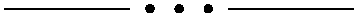
\includegraphics[width=0.35\linewidth,artifact]{ornament}\par}%
\endgroup

\noindent The first image above is a picture of words, so a screen reader says ``Clemson
University'' instead of naming a file. The rule below it is decoration: it is marked as
an artifact and is not in the tag tree at all.
\subsection{Complex images and long descriptions}
\label{sec:longdesc}
A chart, a map or a diagram carries more than one sentence of meaning. Give it a short
\verb|alt| that states its point and says where the rest is, then write the full description
into the document, where every reader can find it. Keep the description beside the figure
when it runs to a few sentences; move it to an appendix when it is long or when many figures
need one.

% A complex image: alt states the point and says where the description is, and
% the same numbers follow as text and as a table. No width key: scaling a
% vector graphic scales the type inside it, and 0.62\linewidth took this
% chart's 9 pt labels down to 6.9 pt, so it is placed at its natural size.
% Meets: Tagged PDF BPG 1.0.1 5.5.2 (Alt); Clemson text concept (9 pt floor).
\begin{figure}\centering
  \caption[Visitors to four South Carolina destinations]{Visitors to four South
    Carolina destinations, 2025. Described in the paragraph below}\label{fig:chart}
  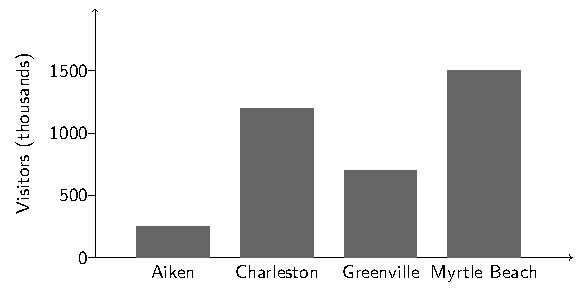
\includegraphics[alt={Bar chart of visitors to four South Carolina destinations: Myrtle Beach draws the most and Aiken the fewest. Described in the paragraph and the table below.}]{chart}
\end{figure}

\noindent \strong{Description of \autoref{fig:chart}.} The horizontal axis names four
destinations. The vertical axis is ``Visitors (thousands)'' and runs from 0 to 1500. Aiken had
250 thousand visitors, Charleston 1200, Greenville 700 and Myrtle Beach 1500. The two coastal
destinations drew more visitors than the two inland ones, and Myrtle Beach drew six times as
many as Aiken. \autoref{tab:chartdata} lists the same numbers.

% The data behind a chart is the description a reader can check, so print it as
% a real table with a header row and a header column, not as a picture. The
% short title holds no \ref: a reference inside a List of Tables entry would be
% a link inside the entry's own link, which is not a legal pair of tags.
% Meets: ISO 32000-2:2020 14.8.4.8.3 (TH, Scope); WCAG 2.1 1.1.1.
\begin{table}\centering
  \caption[The numbers behind the visitor chart]{The numbers behind
    \autoref{fig:chart}}\label{tab:chartdata}
  \tagpdfsetup{table/header-rows={1}, table/header-columns={1}}
  \begin{tabular}{lr}
    \toprule Destination  & Visitors (thousands) \\ \midrule
    Aiken        & 250 \\
    Charleston   & 1200 \\
    Greenville   & 700 \\
    Myrtle Beach & 1500 \\ \bottomrule
  \end{tabular}
\end{table}
% The other pattern: the caption names the appendix and the appendix entry names
% the figure, so a reader can follow the link either way. \ref is not used inside
% alt, because alt is written to the PDF as a plain string.
% Meets: Tagged PDF BPG 1.0.1 5.5.2; WCAG 2.1 1.1.1.
\begin{figure}\centering
  \caption[The cable wall, described in an appendix]{The cable wall in the
    network store. Full description in \autoref{app:desc}}\label{fig:wall}
  
\includegraphics[width=0.3\linewidth,alt={Photograph of the cable wall. Full description in the appendix Extended image descriptions.}]{cables}
\end{figure}
\subsection{Decorative rules, other languages and abbreviations}
Four small things that come up in any paper; the first two need a command, shown after the list.
% A rule drawn inside a paragraph is decoration, so it is marked as an artifact.
% In Lua mode the artifact state is global, so \tagmcend must be followed at once
% by \tagmcbegin{tag=text}; without it the rest of the paragraph is written as an
% artifact and disappears from the tag tree. \tagmcbegin/\tagmcend are the
% documented tagpdf commands for this, and nothing higher level covers a rule.
% Meets: ISO 32000-2:2020 14.8.2.2 (artifacts); Tagged PDF BPG 1.0.1 4.3.1.
\begin{description}
  \item[A decorative rule] A rule that only separates words carries no meaning:
    \tagmcbegin{artifact}\rule{2cm}{0.4pt}\tagmcend%
    \tagmcbegin{tag=text} and the sentence carries on after it.
  % A phrase in another language needs its own /Lang so a screen reader changes
  % voice. babel is the usual way, but its language files are reported as
  % incompatible with tagging, and \foreignlanguage writes no /Lang. The kernel's
  % inline tagging socket (the one \emph uses) opens a Span with its own marked
  % content, then reopens the paragraph's, so no text before or after it is lost.
  % Meets: ISO 32000-2:2020 14.9.2 (Lang); WCAG 2.1 3.1.2 (language of parts).
  \item[A phrase in another language] The French for ``right away'' is
    \UseTaggingSocket{inline/begin}{tag=Span,lang=fr-FR}%
    tout de suite\UseTaggingSocket{inline/end}, tagged as a Span whose language is French.
  \item[An abbreviation] Write it out the first time it appears: Institutional Review Board
    (IRB). PDF has an \verb|/E| attribute for an expansion, but it is not needed once the
    expansion is in the text, where every reader gets it.
  \item[Color] Color is never the only signal. \autoref{fig:chart} draws every bar in one
    shade and names each bar on the axis, so nothing depends on telling colors apart.
\end{description}

\noindent The commands behind the first two items, copied from the source of this file:
\begin{verbatim}
\tagmcbegin{artifact}\rule{2cm}{0.4pt}\tagmcend%
\tagmcbegin{tag=text}
\UseTaggingSocket{inline/begin}{tag=Span,lang=fr-FR}%
tout de suite\UseTaggingSocket{inline/end}
\end{verbatim}
\section{Tables}
\label{sec:tables}
A table is accessible when a reader can tell which cells are headers and what each header
covers. Declare the header cells with \verb|\tagpdfsetup| before \verb|\begin{tabular}|, put the
caption above the table, as above every figure in this file, and keep notes outside it. The
eight layouts below, and the one caveat that follows them, cover the cases that come up in a
thesis.

% Layouts follow https://www.clemson.edu/accessibility/digital/concepts/tables.html
% Rules: the caption goes above the table, as the Graduate School's Word template
% has it; declare the header row and/or column; a merged cell must carry its
% span; notes stay outside the table; avoid empty cells; never nest tables.
% Meets: ISO 32000-2:2020 14.8.4.8.3 (TH, Scope); Tagged PDF BPG 1.0.1 4.2.6.2.

% 1. Simple table, header row: every cell in row 1 is a TH with Scope=Column.
\begin{table}\centering
  \caption{Simple table: the first row is the header (column scope)}\label{tab:headerrow}
  \tagpdfsetup{table/header-rows={1}}
  \begin{tabular}{lrr}
    \toprule Item & Count & Share \\ \midrule
    Alpha & 12 & 40\% \\
    Beta  & 18 & 60\% \\ \bottomrule
  \end{tabular}
\end{table}
% 2. Simple table, header column: every cell in column 1 is a TH with Scope=Row.
\begin{table}\centering
  \caption[Simple table: the first column is the header]{Simple table: the first
    column is the header (row scope); the three data columns are trials 1 to 3}
  \tagpdfsetup{table/header-columns={1}}
  \begin{tabular}{lrrr}
    \toprule
    Mean     & 4.1 & 4.4 & 4.0 \\
    Median   & 4.0 & 4.5 & 3.9 \\
    Std.\ dev. & 0.6 & 0.5 & 0.7 \\ \bottomrule
  \end{tabular}
\end{table}
% 3. Header row and header column: the top-left cell gets Scope=Both.
\begin{table}\centering
  \caption{Header row and header column (the corner cell has both scopes)}
  \tagpdfsetup{table/header-rows={1}, table/header-columns={1}}
  \begin{tabular}{lrrr}
    \toprule Statistic  & Trial 1 & Trial 2 & Trial 3 \\ \midrule
    Mean       & 4.1 & 4.4 & 4.0 \\
    Median     & 4.0 & 4.5 & 3.9 \\ \bottomrule
  \end{tabular}
\end{table}
% 4. Complex table, multi-level header: two header rows; \multicolumn cells get
% ColSpan automatically. table/multirow=2 makes the corner cell span both rows,
% so the blank cell under it is not an empty header (leave that cell empty).
% header-columns={1} as well: without it the row labels are data cells and every
% number names its two column headers but not its method.
% Meets: ISO 32000-2:2020 14.8.4.8.3 (Headers, Scope); Clemson complex tables.
\begin{table}\centering
  \caption{Complex table: a two-level header with merged header cells}
  \tagpdfsetup{table/header-rows={1,2}, table/header-columns={1}}
  \begin{tabular}{lcccc}
    \toprule
    \tagpdfsetup{table/multirow=2}%
    Method & \multicolumn{2}{c}{Training set} & \multicolumn{2}{c}{Test set} \\
           & Precision & Recall & Precision & Recall \\
    \midrule
    Baseline & 0.74 & 0.68 & 0.71 & 0.64 \\
    Proposed & 0.91 & 0.86 & 0.88 & 0.81 \\ \bottomrule
  \end{tabular}
\end{table}
% 5. Complex table, merged data and header cells: a row header spanning two rows
% (table/multirow=2, RowSpan=2) and a data cell spanning two columns (ColSpan=2).
% A cell spanning rows AND columns takes the key inside the \multicolumn text:
% \multicolumn{2}{l}{\tagpdfsetup{table/multirow=2}Text}; before it, it aborts.
\begin{table}\centering
  \caption{Complex table: merged cells carry their row and column spans}
  \tagpdfsetup{table/header-rows={1}, table/header-columns={1}}
  \begin{tabular}{llrr}
    \toprule Group & Sample & Before & After \\ \midrule
    \tagpdfsetup{table/multirow=2}%
    Control   & S1 & 10 & 11 \\
              & S2 & 12 & 12 \\
    \tagpdfsetup{table/multirow=2}%
    Treatment & S3 & 10 & 15 \\
              & S4 & \multicolumn{2}{c}{not measured} \\ \bottomrule
  \end{tabular}
\end{table}
% 6. Headers outside the first row. A group row ("Fall semester") in the middle
% of a table is a header row too (table/header-rows={1,2,5}, one \multicolumn
% cell per group), but the /Headers the package writes under a second group
% still name the first group, so a screen reader would hear the wrong group.
% Until that is fixed, do what Clemson recommends anyway: one table per group.
\begin{table}\centering
  \caption{One table per group: fall semester}
  \tagpdfsetup{table/header-rows={1}, table/header-columns={1}}
  \begin{tabular}{lrr}
    \toprule Course   & Enrolled & Passed \\ \midrule
    MATH 101 & 120 & 108 \\
    MATH 102 & 95  & 90  \\ \bottomrule
  \end{tabular}
\end{table}
\begin{table}\centering
  \caption{One table per group: spring semester}
  \tagpdfsetup{table/header-rows={1}, table/header-columns={1}}
  \begin{tabular}{lrr}
    \toprule Course   & Enrolled & Passed \\ \midrule
    MATH 101 & 130 & 121 \\
    MATH 102 & 88  & 80  \\ \bottomrule
  \end{tabular}
\end{table}
% 7. Title and notes outside the table; no empty data cells. The \caption is the
% title and its short form is what the List of Tables prints; a note is a paragraph
% after the table, not a row inside it; a cell with no value says so ("n/a").
\begin{table}\centering
  \caption[A table with no empty cells]{A table with no empty cells; its note
    follows as a paragraph}
  \tagpdfsetup{table/header-rows={1}}
  \begin{tabular}{lrr}
    \toprule Site & 2024 & 2025 \\ \midrule
    North & 41 & 45 \\
    South & n/a & 39 \\ \bottomrule
  \end{tabular}
\end{table}
\noindent Note: the South site opened in 2025, so it has no 2024 value.

% The caveat, not a layout: a table that runs over a page break. longtable typesets
% its caption as a table row, tagged as a header cell rather than a Caption, so
% split a long table into page-sized tables, each with its own \caption. A wide
% table turned sideways is not shown: lscape and pdflscape are untested here.

The grid of names below holds no data and no headers: it only puts two names side by side. It
is not a table, so table tagging is switched off for it and a screen reader reads the names
as plain text rather than announcing rows and columns. Better still, lay such text out without
a \texttt{tabular}.

% 8. A layout grid is not a data table: switch table tagging off for it so no
% Table, TH or TD is written and the words stay ordinary text (Acrobat fails a
% Table without headers and ignores the PDF 2.0 presentation role). Keep
% table/tagging=false inside a group: left open, it would untag every later table.
% Meets: ISO 32000-2:2020 14.8.4.8 (Table); Clemson tables concept.
\begingroup\centering
\tagpdfsetup{table/tagging=false}%
\begin{tabular}{cc}
  First Author & Second Author \\
  Clemson University & Clemson University
\end{tabular}\par
\endgroup
\noindent Never nest a table inside a table; split it into two tables instead.
\section{Footnotes and endnotes}
A footnote belongs at the foot of the page it is read on; an endnote is collected and printed
with the others near the end. A footnote is tagged as a note with a two-way reference to its
mark; an endnote is an item in a tagged list whose number links back to the mark, and the
mark links to the note, so a reader can follow either and come straight back. Footnote marks
are arabic and endnote marks roman, so the two series cannot be confused.

% Endnotes: enotez. Its mark is a link to the note and the note's number is a
% link back, and the list is tagged L/LI/Lbl/LBody. Rejected: the endnotes
% package (plain superscript marks, no Link and no Ref, so the note cannot be
% reached), and hand-rolled \hypertarget/\hyperlink pairs (a Link both ways, but
% the note list is ordinary text with no note structure and no Ref attribute).
% The class loads and configures enotez. Meets: ISO 32000-2:2020 14.8.4.7 (Link).
Write a footnote where it is needed, with \verb|\footnote{...}|,\footnote{The second
footnote in the file; its mark is the arabic 2.} and an endnote in the same place in the
text, with \verb|\endnote{...}|.\endnote{The second endnote. Inside a note, write
commands with \texttt{\textbackslash texttt}, because \texttt{\textbackslash verb} reads
its own text and cannot sit inside the argument of another command.}
\appendix
% In the article class \appendix letters the sections but leaves floats numbered
% straight through. \counterwithin adds the section letter and restarts the count,
% so this appendix holds Table A.1 and Figure A.1, as the Word template has it.
\counterwithin{figure}{section}
\counterwithin{table}{section}
\section{An appendix}
\label{app:example}
An appendix holds material that supports the text but would interrupt it: survey instruments,
long tables of results, proofs, source code. Its sections are lettered, its figures and
tables are numbered A.1, B.1 and so on, and it appears in the table of contents like any
other section. Tables and figures in an appendix are tagged exactly as in the body.

\begin{table}\centering
  \caption{A table in an appendix, numbered A.1}
  \tagpdfsetup{table/header-rows={1}}
  \begin{tabular}{lr}
    \toprule Instrument & Responses \\ \midrule
    Survey A & 412 \\
    Survey B & 385 \\ \bottomrule
  \end{tabular}
\end{table}

\begin{figure}\centering
  \caption{A figure in an appendix, numbered A.1}
  
\includegraphics[width=0.35\linewidth,alt={Coiled gray network cables on a beige pegboard wall, shown again here as an example of a figure inside an appendix.}]{cables}
\end{figure}
\section{Extended image descriptions}
\label{app:desc}
This appendix holds the descriptions that are too long to sit beside their figures.
Begin every entry with the figure it describes, so that the caption and the description
link to each other in both directions.

\strong{\autoref{fig:wall}:} A color photograph of a storage wall in a network room. Gray
patch cables are wound into loops about twenty centimetres across and hung on a beige
pegboard in six rows of eight. A blue plastic clip holds each coil near the top, and the blue
connectors at the ends of each cable hang below the coil. The rows are evenly spaced and the
coils are of much the same size, so the wall reads as a store of unused cable rather than as
equipment in service.

% The endnotes are printed after the appendices and before the works cited, where
% a reader looks for them. \printendnotes also adds "Notes" to the contents.
\printendnotes

% The bibliography heading is a starred section, so \phantomsection puts a link
% target here and \addcontentsline lists it. Meets: ISO 32000-2:2020 14.8.4.6.
\phantomsection
\addcontentsline{toc}{section}{\refname}
\bibliographystyle{plain}
\bibliography{references}
\end{document}
